% For plaintext use only
\documentclass[a4paper,notitlepage]{article}

\usepackage{xltxtra}
\usepackage{amsmath}
\usepackage{amssymb}
\usepackage{amsthm}
\usepackage{tikz}
\usepackage{unicode-math}
\usepackage{fontspec}
\usepackage{faktor}
\setmathfont{xits-math.otf}
\usetikzlibrary{positioning}
\usepackage{multicol}

\newtheorem{observation}{Observation}
\newtheorem{proposition}{Proposition}
\newtheorem{definition}{Definition}

\tikzset{node distance=2cm, auto}

\author{Víctor López Juan}
\title{Chapter 4}

\begin{document}
\maketitle
\begin{enumerate}
  \item[4.]

    {\em Use the Eckmann-Hilton argument to prove that every monoid in the
category of groups is an internal group.}

    Let $\left ( \vert G \vert, ·, 1_G \right)$ be an object
    in {\bf Grp}. We define the following monoid in that category.

    The terminal object $1$ is the trivial one-element group.

      
    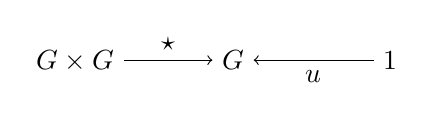
\begin{tikzpicture}
      \node  (GG) {$G \times G$} ;
      \node  (G) [right of=GG] {$G$};
      \node  (T) [right of=G] {$1$};
      
      \draw[->] (GG) to node {$\star$} (G);
      \draw[->] (T) to node {$u$} (G);
    \end{tikzpicture}

    The monoid operation must be associative, and $u$ must behave
    as the unit element.
    
    \begin{multicols}{2}
      
    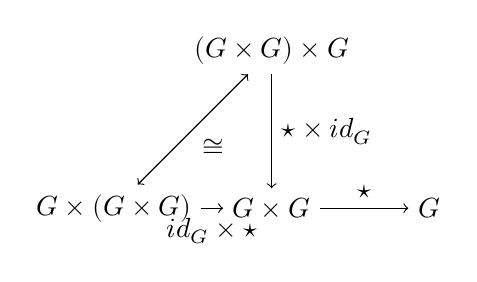
\begin{tikzpicture}
      \node (GGG1) {$(G \times G) \times G$};
      \node (GG)   [below of=GGG1] {$G \times G$};
      \node (GGG2) [left of=GG] {$G \times (G \times G)$};
      \node (G)    [right of=GG]   {$G$};

      \draw[<->] (GGG1) to node {$\cong$} (GGG2); 
      \draw[->] (GGG1) to node {$\star \times id_G$} (GG);
      \draw[->] (GGG2) to node[below] {$id_G \times \star$} (GG);
      \draw[->] (GG) to node {$\star$} (G);
    \end{tikzpicture}

    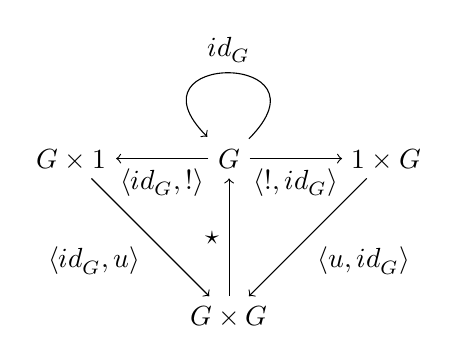
\begin{tikzpicture}
      \node (G) {$G$};
      \node (UG) [right of=G] {$1 \times G$};
      \node (GU) [left of=G] {$G \times 1$};
      \node (GG) [below of=G] {$G \times G$};

      \path (G) edge [loop] node [above] {$id_G$} (G); 
      
      \draw[->,swap] (G) to node {$\langle ! , id_G \rangle$} (UG);
      \draw[->] (G) to node {$\langle  id_G, ! \rangle$} (GU);
      \draw[->] (UG) to node {$\langle  u, id_G \rangle$} (GG);
      \draw[->,swap] (GU) to node {$\langle  id_G, u \rangle$} (GG);
      \draw[->] (GG) to node {$\star$} (G);
    \end{tikzpicture}
    
    \end{multicols}
      
    Observe that $\vert G \times G \vert = \vert G \vert \times \vert G \vert$.
    By applying the forgetful functor $\vert · \vert$ : {\bf Grp} → {\bf Set} to each of
    the three diagrams, we obtain three new diagrams that define a monoid in {\bf Set}.
    Monoids in {\bf Set} are monoids, so the operation $\star$ is associative, and has identity
    element $u(1)$.

    The is defined in {\bf Grp}. This means that the
    arrow $\star$ is a group homomorphism, so the following holds:

        $$\star(g₁·h₁, g₂·h₂) = \star((g₁,g₂)·(h₁,h₂)) = \star(g₁,g₂)·\star(h₁,h₂)$$

    By the {\em Eckmann-Hilton argument}, it follows that the operation
    $\star$ for the monoid is the same as the operation $·$ for the
    group $G$; and this operation is commutative. Therefore,
    monoids in {\bf Grp} are abelian groups.

    Now, we define $i : G → G$, $i(a) = a^{-1}$.
    In general, $i$ is not a group homomorphism, but it is the case if
    $G$ is abelian\footnote{Indeed, $i$ is an automorphism iff the
      group is abelian.

      $$x \cdot y = i(x^{-1}) \cdot i(y^{-1}) = i(x^{-1}\cdot y^{-1}) = (x^{-1} \cdot y^{-1})^{-1} = y\cdot x$$
    }.

    $$i(x^{-1}\cdot y) = (x^{-1}\cdot y)^{-1} = y^{-1} \cdot x = x \cdot y^{-1} = i(x)^{-1} \cdot i(y)$$

    Together with $\star$ and $u$, $i$ defines an internal group.
      
    \begin{tikzpicture}
      \node  (GG)  {$G \times G$};
      \node  (G) [right of=GG] {$G$};
      \node  (T) [right of=G] {$1$};
      \node  (GI) [below of=G] {$G$};
      
      \draw[->] (GG) to node {$\star$} (G);
      \draw[->] (T) to node {$u$} (G);
      \draw[->] (GI) to node {$i$} (G);
    \end{tikzpicture}

  \item[7.]

    Let $\sim$ be a congruence.

    Let $f, f^\prime : A → B$, $f \sim f^\prime$. Also, let $g, g^\prime : B → C$,
    $g \sim g^\prime$.

    Then,

    \begin{align*}
        f^\prime \circ g^\prime &= (id_A \circ f^\prime \circ g^\prime) \circ id_C     \\ 
      &= (id_A \circ f \circ g^\prime) \circ id_C         \tag{$f^\prime \sim f$} \\ 
      &= (f \circ g^\prime \circ id_C)                    \\
      &= (f \circ g \circ id_C)                                 \tag{$g^\prime \sim g$} \\ 
      &= f \circ g                                      \\ 
    \end{align*}

    $$\therefore f^\prime \circ g^\prime \sim f \circ g$$
    
  \item[8.]

    \begin{definition}
      Given functors $F, G : \text{\bf C} → \text{\bf D}$ such that for all
      $C ∈ \text{\bf C}$, $FC = GC$, we define $\sim \subset \text{\bf D}_1 × \text{\bf D}_1$ as follows:
      
    \begin{eqnarray*}{rcl}
       f \sim g \equiv &        & dom(f) = dom(g) \\
                       & \wedge & cod(f) = cod(g) \\
                       & \wedge & \forall \text{\bf E} \forall H : \text{\bf D} → \text{\bf E} : HF = HG ⇒ H(f) = H(g) \\
    \end{eqnarray*}
      
      \end{definition}

    \begin{observation}\label{obs:eq-alpha}
    For every $\alpha \in \text{\bf C}$, $F(\alpha) \sim G(\alpha)$.
    \end{observation}
    \begin{proof}
      Let $f = Fα$, $g = Gα$.
      $$dom(f) = dom(Fα) = F(dom(α)) = G(dom(α)) = dom(Gα) = dom(g)$$
      $$cod(f) = cod(Fα) = F(cod(α)) = G(cod(α)) = cod(Gα) = cod(g)$$

      For any functor F, if $HF = HG$, then $H(f) = HFα = HGα = H(g)$
    \end{proof}

    The equivalence relation $\sim$ can be described as “gluing
    together” arrows in $\text{\bf D}$ using functors $F$ and $G$.

    \begin{proposition}
    $\sim$ is a congruence.
    \end{proposition}
    \begin{proof}

      A congruence relation is an equivalence relation on arrows which
      respects domain, codomain, and composition.

    \begin{itemize}
      \item From reflexivity, symmetry and transitivity for equality
        it follows that $\sim$ is an equivalence relation.           

          \item By definition of $\sim$:

            $$f ~ g \Rightarrow dom(f) = dom(g) \wedge cod(f) = cod(g)$$ 

        \item
          Let $f , g : X → Y$ such that $f \sim g$, and let $a$, $b$ be arbitrary
          arrows $a : A → X$, $b : Y → B$.

          \begin{itemize}

           \item Domains and codomains match.

               $$dom(bfa) = dom(b) = dom(bga)$$
               $$cod(bfa) = cod(a) = cod(bga)$$

            \item
              
              Let $H : D → E$ such that $HF = HG$.

              By defintion of $f \sim g$, $H(f) = H(g)$.

              As a consequence:

              $$H(bfa) = H(b)H(f)H(a) = H(b)H(g)H(a) = H(bga)$$
              
          \end{itemize}

          $$ \therefore bfa \sim bga $$
    \end{itemize}

    Therefore $\sim$ defines a congruence relation.
    In particular, the composition of congruent arrows is congruent
    (see exercise 7).

    \end{proof}

    \begin{proposition}
    The object $\faktor{D}{\sim}$ is the coequalizer of $F$ and
    $G$ in {\bf Cat}.
    \end{proposition}

    \begin{proof}

       Let $P : D → \faktor{D}{\sim}$ be the canonical projection
       into the quotient, $P(x) = [x]$.

       \begin{itemize}

         \item To prove that $P \circ F = P \circ G$, we need to prove
           the equality for both objects and arrows.
           
          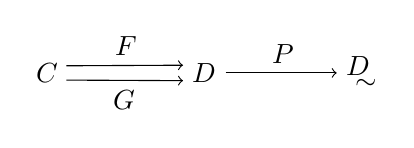
\begin{tikzpicture}
            \node (C) {$C$};
            \node (D) [right of=C] {$D$};
            \node (DQ) [right of=D] {$\faktor{D}{\sim}$};
            
            \draw[->] (C.20) to node {$F$} (D.160);
            \draw[->,swap] (C.340) to node {$G$} (D.200);
            \draw[->] (D) to node {$P$} (DQ);
          \end{tikzpicture}

          \begin{itemize}
            \item For every object $C$ in {\bf C}, $F(C) = G(C)$.
              
              The quotient only applies to arrows; therefore:

              $$\forall C . P(F(C)) = F(C) = G(C) = P(G(C))$$

            \item 

              Let $α \in \text{\bf C}$.

              By observation \ref{obs:eq-alpha}, $Fα \sim Gα$.

              $$P(F(α)) = [Fα] = [Gα] = P(G(α))$$.
         \end{itemize}

        In order to be a coequalizer, $P$ also has to be universal.
        Namely, for any arrow $Z$ as in the following
        diagram, an unique arrow $\overline{Z}$ must exist such that the
        diagram commutes.
          
          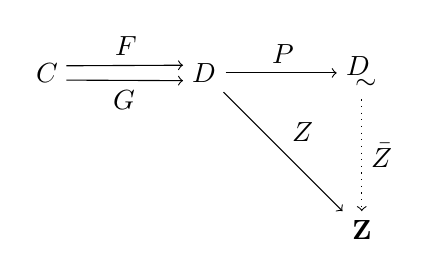
\begin{tikzpicture}
            \node (C) {$C$};
            \node (D) [right of=C] {$D$};
            \node (DQ) [right of=D] {$\faktor{D}{\sim}$};
            \node (Z) [below of=DQ] {$\text{\bf Z}$};
            
            \draw[->] (C.20) to node {$F$} (D.160);
            \draw[->,swap] (C.340) to node {$G$} (D.200);
            \draw[->] (D) to node {$P$} (DQ);
            \draw[->] (D) to node {$Z$} (Z);
            \draw[->,dotted] (DQ) to node {$\bar{Z}$} (Z);
          \end{tikzpicture}

          \begin{description}
            \item[Existence]

              Assume the axiom of choice.
              
              Let $I$ be some choice mapping from $\faktor{D}{\sim} → D$,
              such that, for every arrow $α$, $I([α]) ∈ [α]$; and, for
              any object $C$, $I(C) = C$.

              $$I([α]) ∈ [α] \Rightarrow I([α]) \sim α$$

              Let $\overline{Z} = Z \circ I$. 

              For any object $C$:
              
              $$\overline{Z}(P(C)) = Z(I(P(C))) = Z(I(C)) = Z(C)$$ 

              For any arrow $α$:
              
              \begin{align*}
                    \overline{Z} P(α) &= Z (I P(α)))         && \text{definition of $\overline{Z}$}   \\
                                 &= Z (I [α]))              && \text{definition of $P$}   \\
                                 &= Z (α))                   && \text{$I[α] \sim α, ZF = ZG$}   \\
              \end{align*}  

              Therefore, the diagram above commutes.
                    
             \item[Uniqueness]
                    
                Let $\overline{Z}^\prime : \faktor{D}{\sim} → X$ such
                that $\overline{Z}^\prime \circ P = Z$.

                For any object $C$:

                $$\overline{Z}^\prime(C) = \overline{Z}^\prime(P(C)) = Z(C) = \overline{Z}(P(C)) = \overline{Z}(C)$$ 

                For any arrow $α$:

                $$\overline{Z}^\prime([α]) = \overline{Z}^\prime(P(α)) = Z(α) = \overline{Z}(P(α)) = \overline{Z}([α])$$

                Therefore, $\overline{Z}^\prime = \overline{Z}$.
         
         \end{description}
    \end{itemize}    
  \end{proof}
\end{enumerate}

\end{document}
  
